\documentclass{beamer}
\usepackage[ngerman]{babel}
\usepackage[utf8]{inputenc}
\usepackage{natbib}
\usefonttheme{professionalfonts}
\usetheme{Boadilla}

\begin{document}
\title[Adaptive Gestenerkennung]{Adaptive Gestenerkennung mit Variationsabschätzung für interaktive Systeme}
\author{Maxim Boianetchii \and Marian Stein}
\date{\today}
%\institute{Universität Rostock}

\begin{frame}
\titlepage
\end{frame}

\begin{frame}\frametitle{Motivation}
\begin{itemize}
\item Gestenerkennung in vielen Gebieten gefragt:
\begin{itemize}
\item Medizin
\item Automobilindustrie
\item Unterhaltungsbranche
\end{itemize}
\item Mit aktuellen Methoden nur eingeschränkt möglich
\begin{itemize}
\item Erkennung teilw. nur nach vollst. Ausführung der Geste
\item Keine Rückmeldung von Zusatzinformationen über die Geste(z.B Geschwindigkeit)



\end{itemize}
\end{itemize}
\begin{columns}
\begin{column}{0.4\textwidth}
\begin{figure}
\centering
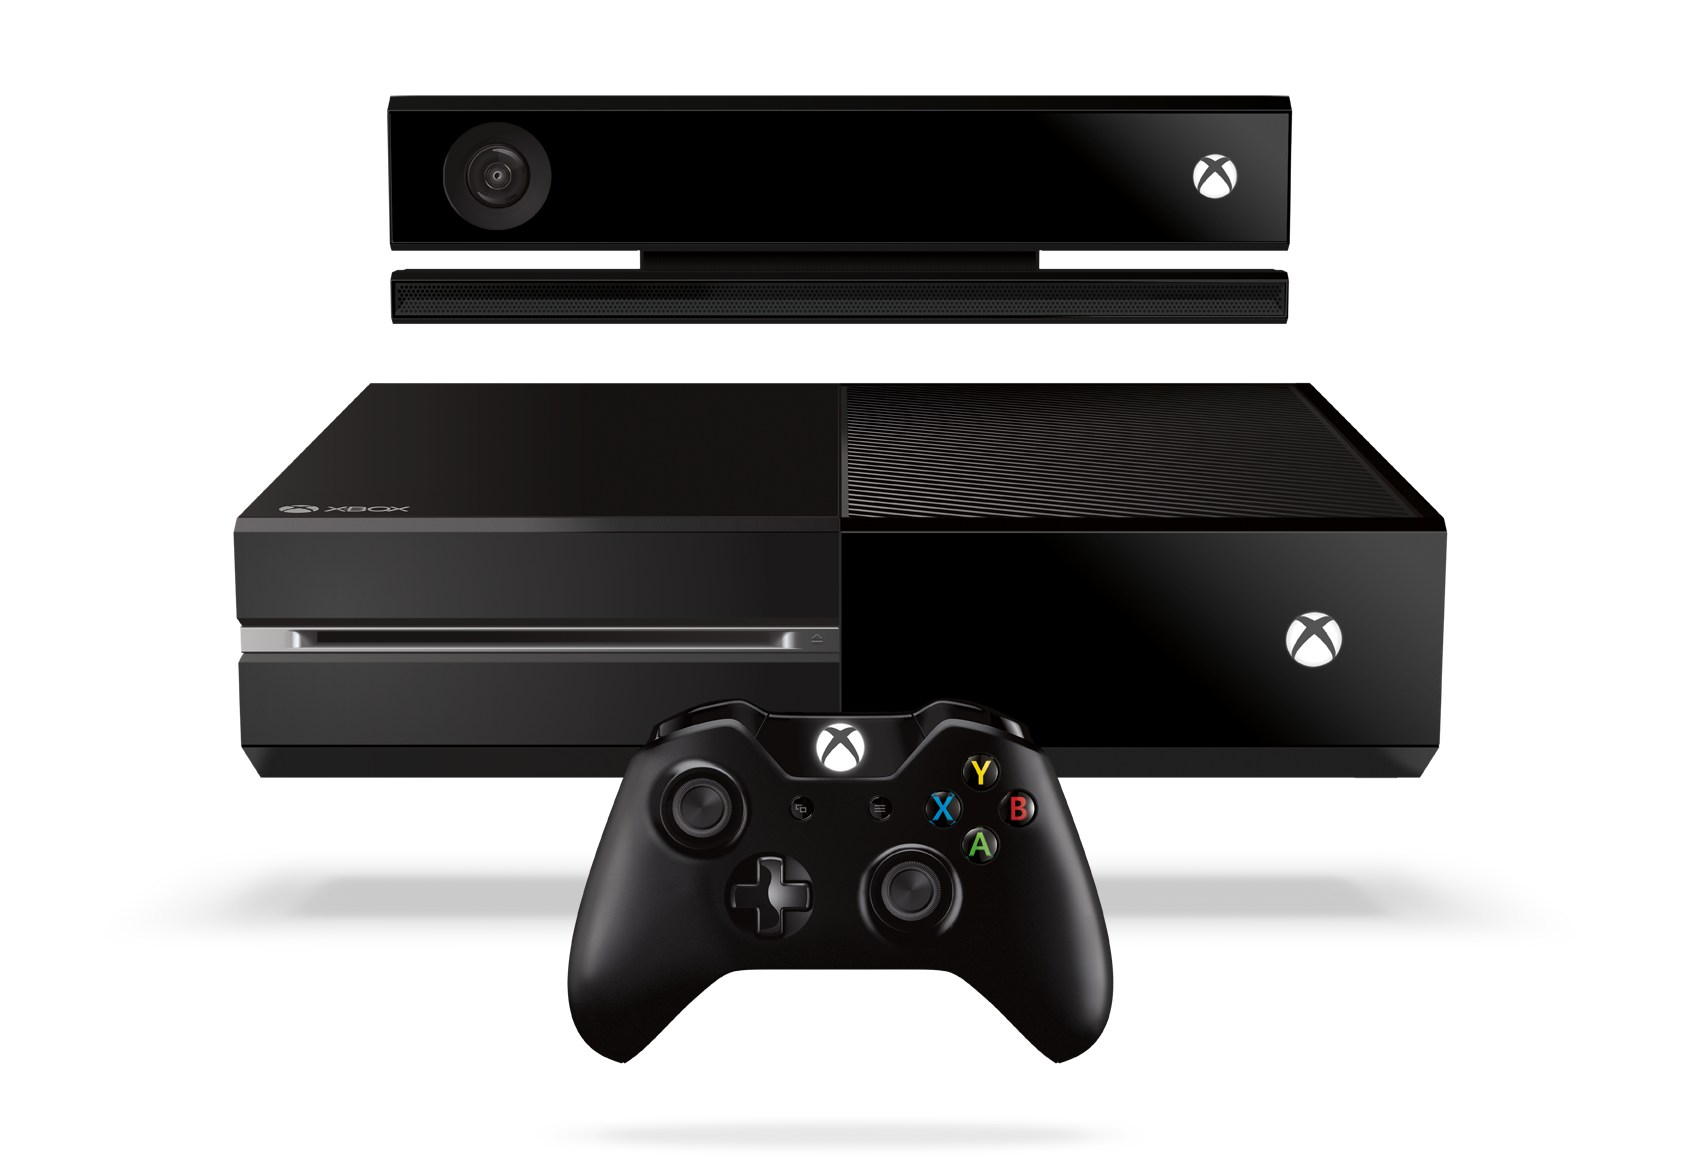
\includegraphics[width=0.7\linewidth]{../Bilder/xbox}
\label{fig:xbox}
\end{figure}
\end{column}
\begin{column}{0.4\textwidth}
\begin{figure}
\centering
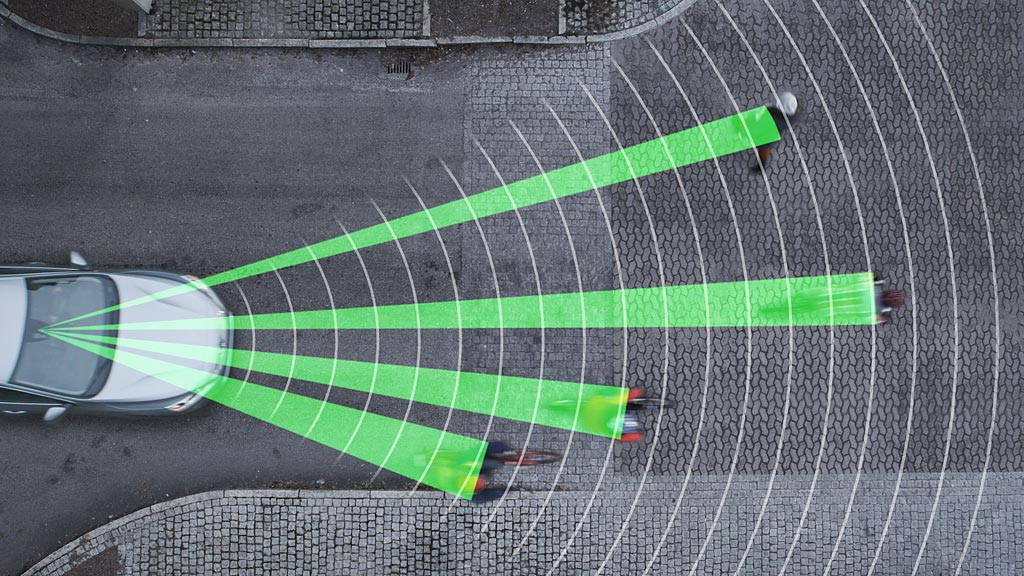
\includegraphics[width=0.7\linewidth]{../Bilder/fussgaenger}
\label{fig:fussgaenger}
\end{figure}
\end{column}
\end{columns}
\end{frame}
\begin{frame}\frametitle{Vorgeschlagene Methode}
\begin{itemize}
\item Verwendung eines Partikelfilters
\item frühzeitige Erkennung und Rückmeldung von Variationsinformationen, z. B. Geschwindigkeit, Drehung, etc.
\begin{itemize}
\item Ermöglicht Anwendungen, bei denen die Benutzer direkt während der Gestenausführung interagieren können
%Verweis auf Nutzerstudie
\end{itemize}
\end{itemize}
\end{frame}
\begin{frame}\frametitle{Ähnliche Arbeiten}
\begin{itemize}
\item \citet{Wobbrock2007}
\end{itemize}
\end{frame}

\begin{frame}\frametitle{Literatur}
\bibliographystyle{plainnat}
\bibliography{praesentation}

\end{frame}

\end{document}